\chapter{Heterogeneous Cooperative Spectrum Sensing (CSS)}
\label{chapter2}

This chapter provides the background information needed to understand the chapters that follows. It examines the basic outlines of a heterogeneous networks and how cooperative spectrum sensing (CSS) can help in enhancing the accuracy of signal source estimation. The fusion center (FC) collects the data from the sensor node network and process it to make the reliable decision. Secondly, this chapter investigates various algorithms which can be used in heterogeneous network to estimate signal source. Finally, it also outlines the necessary hardware and software tools used in the implementation of heterogeneous CSS chapter.

\section{Cognitive Radios}
Cognitive radio (CR)~\cite{cogjm} is a communication systems paradigm that focuses on employing highly agile, environmentally aware, intelligent wireless platforms in
order to autonomously select and configure device operating parameters based on the prevailing radio and network environmental conditions~\cite{bookhtn1}. In general the cognitive radio may be expected to look at parameters such as channel occupancy rate, available channels, bandwidth required for data transmission and the modulation types that may be used. It must also look at the regulatory requirements set by the Federal Comm. In some instances a knowledge of geography and this may alter what it may be allowed to do. Software-defined radios (SDR) are mainly responsible for making cognitive radios used in wireless communications system a reality. Software radios provide a vast untapped potential to personalize services, and they make the process of modifying the radio characteristics extremely simple. 

The work is underway to determine the best possible methods of developing the cognitive radio communications system that can fulfill all its requirements. To facilitate the intelligent decision making capabilities in these cognitive radio systems, machine learning algorithms have been proposed in the literature~\cite{barker2008mission,haykin2005cognitive,newman2007cognitive,newman2008population} to automate the reconfiguration process. The Figure~\ref{cograd} describes the various building blocks of a cognitive radio system. The spectrum sensing is performed to estimate the spectrum holes in the band and after the analysis the decision strategy is prepared. The radio is configured with the new parameters based on the radio environment and the spectrum decision made.  

\begin{figure}[ht!]
	\centering
	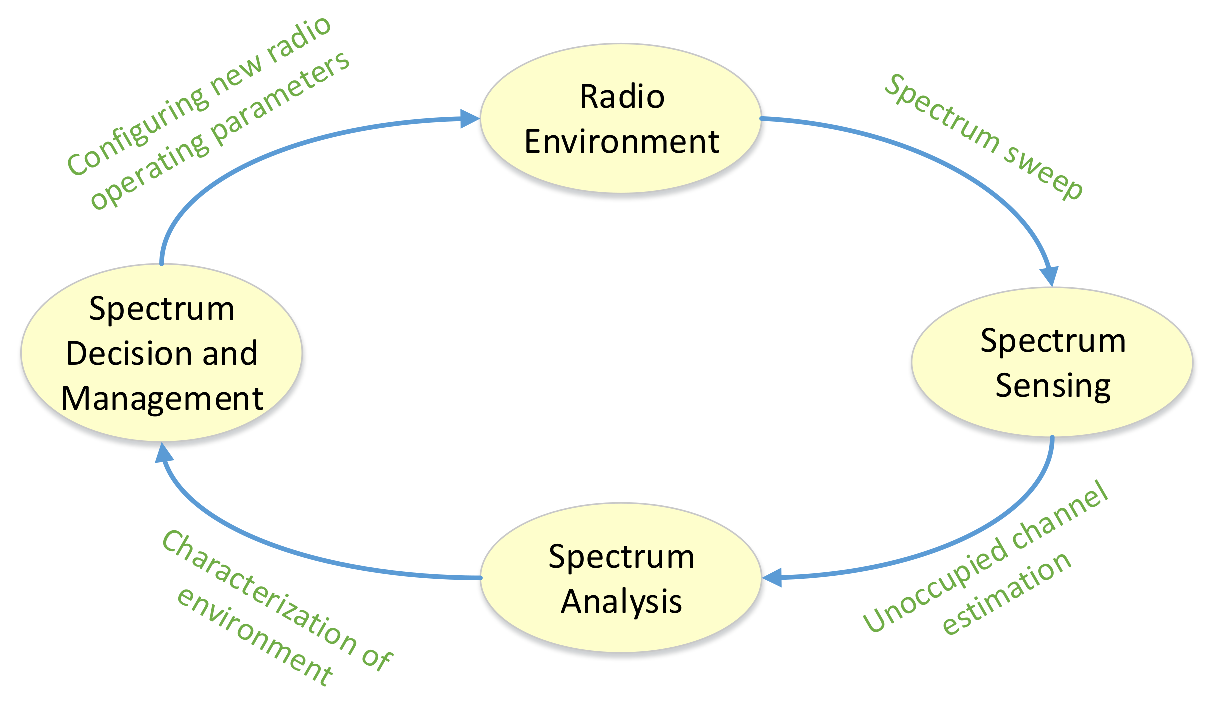
\includegraphics[width=\textwidth,keepaspectratio]{images/Gill/figs/cognitive_radio.eps}
    \caption{The block diagram explaining the basic parts of Cognitive Radio system. The operating parameters are configured based on the characterization of the wireless environment.} 
\label{cograd}      
\end{figure}

\section{Heterogeneous Networks}
Heterogeneous CR network, in which each SU may be equipped with different numbers of antennas and sampling
rates. In addition, each SU may experience distinct channel fading and suffer from different noise levels due to their respective
locations and device performances, such as amplifier and ADC. As a result, each SU may have different sensing capabilities
and reliability values. This is a universal and fundamental characteristic of a heterogeneous CR network, which has not
been taken into account in any previously proposed cooperative spectrum sensing schemes.[GuoshengYangHetNetPaper]

\section{Cooperative Spectrum Sensing}
Cooperative sensing (CS) with soft combination, i.e., multiple SUs sense the common signal in a coordinated mode,
has been proven to be more reliable than single SU sensing [4]–[13] under a practical fading environment. For its low
implementation complexity, energy detection (ED)-based cooperative spectrum sensing has been widely investigated in recent
years. In particular, the maximum ratio combining (MRC) and the square-law combining (SLC) have been studied in [9]
and [12]. However, the MRC scheme needs the channel state information (CSI) from the PU to the SUs and from each SU
to the fusion center (FC). If the SLC scheme is applied with a variable amplification factor at each SU, the CSI from the PU
to the SUs and from the SUs to the FC are also needed. As a result, both MRC and SLC schemes have substantially high
complexity. In contrast, cooperative ED with equal gain combination (EGC) is often considered in practical implementation
due to its low complexity [9], [13].[GuoshengYangHetNetPaper]


\section{Software Defined Radios}
Now that the signal processing techniques have been discussed, a platform for implementation is needed. The alley chosen for this thesis is to utilize a new hardware frontier
called Software-Defined Radio, which will be discussed in this section.

\begin{figure}[ht!]
	\centering
	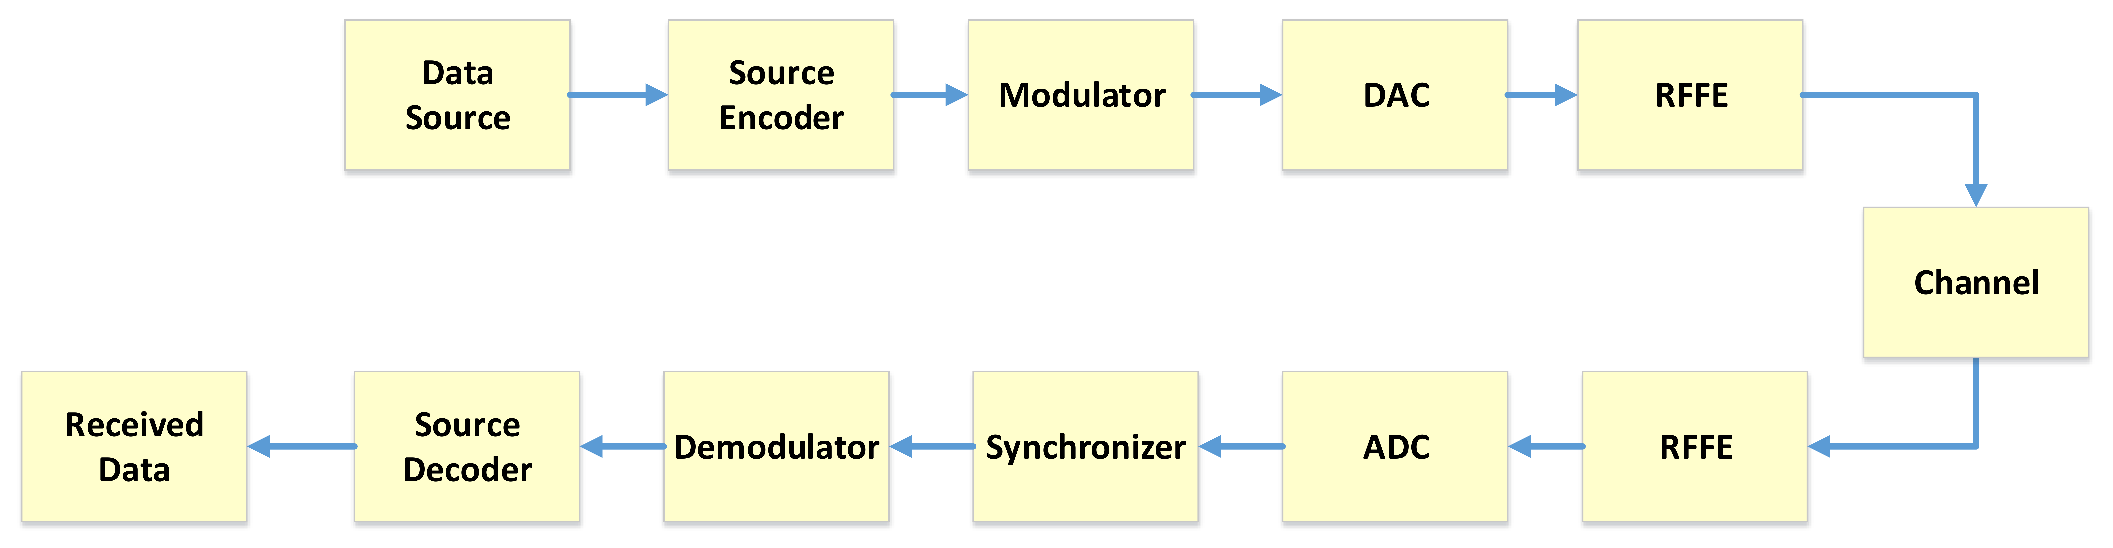
\includegraphics[width=\textwidth,keepaspectratio]{images/Gill/figs/softwaredefinedradio.eps}
    \caption{Software defined radio pushes all the adaptive elements and data manipulation operation into software. The goal of SDR is to provide or define all of the radio operation in software.} 
\label{sdr}      
\end{figure}

For the past two decades there has been a paradigm shift is the definition of a radio device. The conversation has to do with the question of where hardware ends and where
software begins. The term Software Defined Radio, coined by Dr. J. Mitola III, defined as a set of digital signal processing (DSP) primitives, a meta-level system for combining
the primitives into communication system functions (transmitter, channel model, receiver, etc.), and a set of target processors on which the software radio is hosted for real-time
communications [42]. Dr. Mitola understood how software provided the flexibility that hardware never could, and as time made it more mailable SDR would become dominant.

SDRs can be flexible enough to avoid the “limited spectrum” assumptions of designers of previous kinds of radios, in one or more ways including: Ultrawideband transceivers, cogni-
tive radio, dynamic mesh networks, software-defined antenna arrays among others [43]. One of the first SDR implementations was a project called “SpeakEasy”. The original purpose of
SpeakEasy was to use programmable processing to emulate more than ten existing military radios, operating in frequency bands between 2 MHz and 2 GHz [44]. Therefore with this
single radio, the operator could talk to ten radios operating under ten different standards. As simple enough idea, but unfortunately the implementation left much to be desired. For
example, physically the device encapsulated the entire back of a common pickup truck [44]. This might be great for a ground station that does not move, but for a mobile unit this
was highly impractical. Secondly, in 1992 field programmable gate arrays (FPGA) required significant time, comparatively to re-flash or change their operational parameters. Again,
this also limited SpeakEasy’s flexibility.[Travisthesis].
\subsection{Universal Software Radio Peripheral (USRP) N210}

\begin{figure}[ht!]
	\centering
	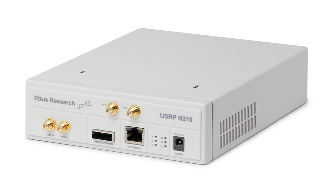
\includegraphics[width=\textwidth,keepaspectratio]{images/Gill/figs/usrp.eps}
    \caption{USRP N210.} 
\label{usrp}      
\end{figure}

\subsection{RTL-SDR Software-Defined Radio}

\begin{figure}[ht!]
	\centering
	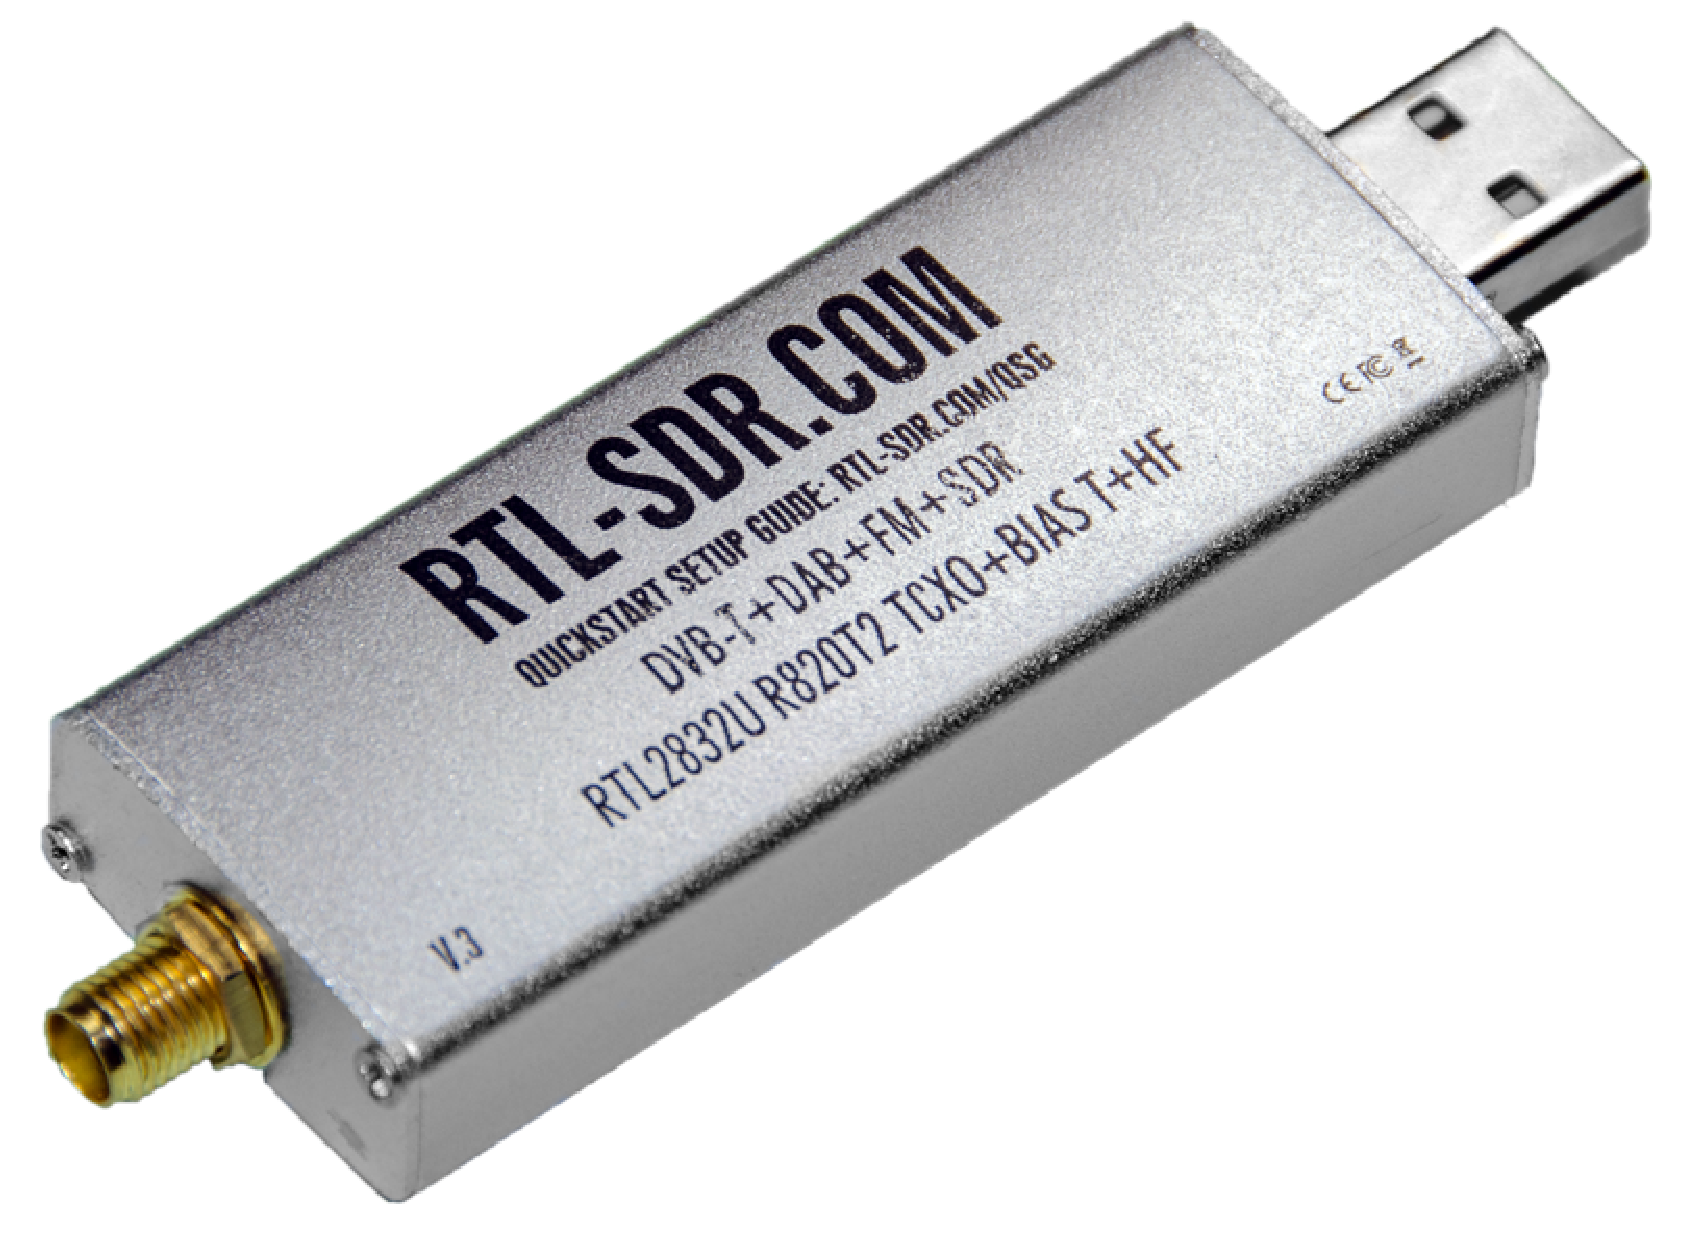
\includegraphics[width=\textwidth,keepaspectratio]{images/Gill/figs/rtlsdr.eps}
    \caption{RTL-SDR R2832u} 
\label{rtlsdr}      
\end{figure}

\subsection{GNURadio and Software-Defined Radio}
The first software package to be discussed by this thesis is GNU Radio. GNU Radio provides the reconfigurable signal processing blocks that are necessary for software defined
radios. GNU Radio is an open source project allowing for SDR developers to develop unique signal processing blocks and SDR systems. GNU Radio was started in 2001, originally
forked from the SpectrumWare project developed at the Massachusetts Institute of Technology [46]. Since 2001, the code base has undergone massive changes, containing almost
no code from the original SpectrumWare project. Physically the code consist of three languages Python, C++, and SWIG. Python provides the overarching control of the system or
program, while C++ provides the actual signal processing blocks and mathematics. SWIG is a wrapper for C++ which allows Python to dynamically wrap around C++ and control
or compile with it. A diagram below better illustrates this architecture. It is also important to mention that there as significant paradigm shifts in the community, pushing more and more code to Python rather than C++, due to its easier programming syntax and structure.

\begin{figure}[ht!]
	\centering
	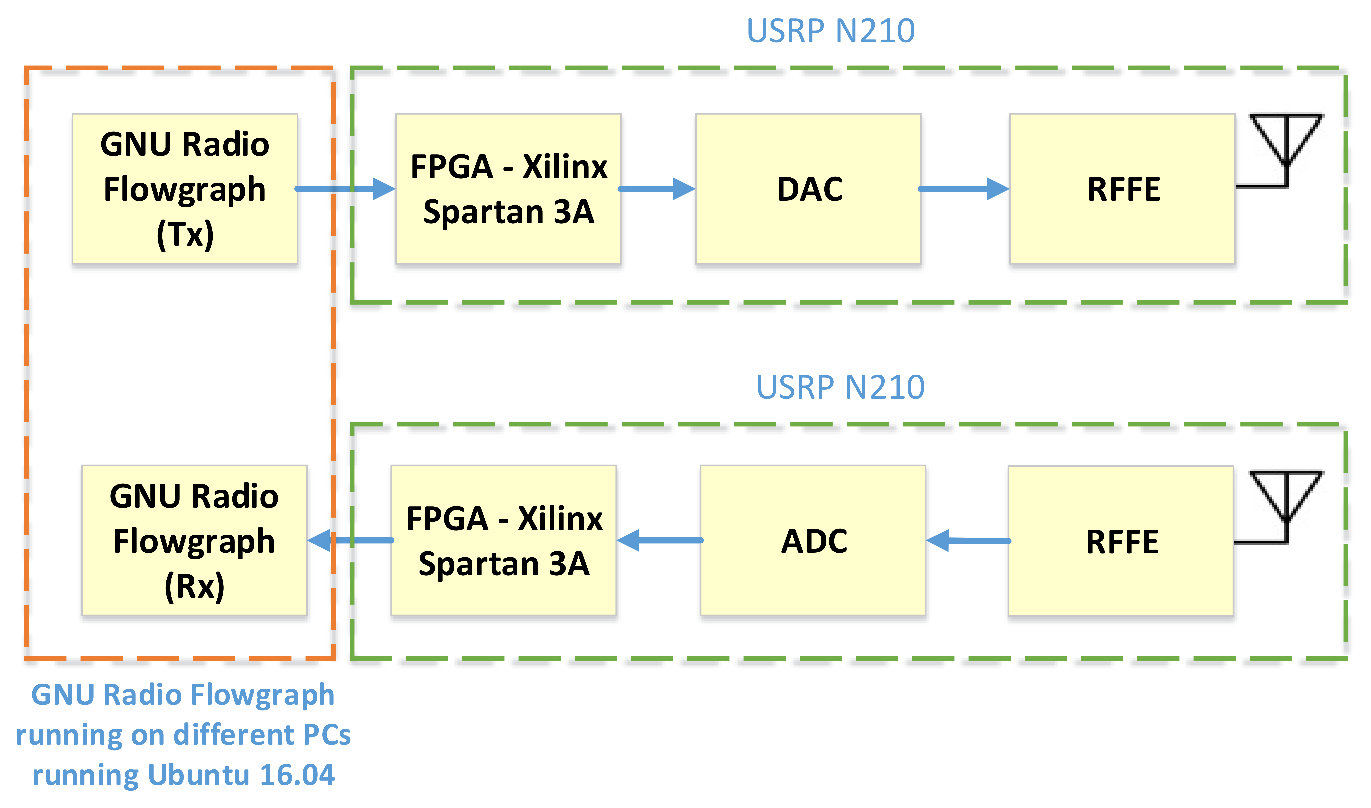
\includegraphics[width=\textwidth,keepaspectratio]{images/Gill/figs/gnuradio.eps}
    \caption{GNURadio and Software-Defined Radio} 
\label{gnuradio}      
\end{figure}

GNU Radio provides a very structured framework of flow design. Data processing segments are extremely self contained to minimize error propagation during system debugging.
Since the software is open-source full access to all code is provide, giving low-level access to all operation within GNU Radio. Much of the actions have been abstracted to limited the
knowledge of the lower layers, but if specific actions are required for an application. Then serious depth or knowledge is needed about the overall project’s structure, which is quite
overloading.[Travisthesis]


\subsection{MATLAB}
MATLAB is an extremely well known engineering, mathematical, biological, and financial software suite. MATLAB provide massive data leverage and advanced communication
system models and algorithm for significant data processing. Since 2007, they have also provided hardware compliance with specific SDR platforms through their Simulink plat-
form, and more recently within MATLAB itself [47]. This thesis primarily utilizes the signal processing and communication system aspects of MATLAB, since MATLAB cannot
fully utilize all aspects of the chosen hardware. It is important to note under alternate constraints, MATLAB can provide adequate performance directly interfacing with hard-
ware, especially when accessing its targeting features seen here [48]. Figure 2.10 shows an example of a common MATLAB SDR model through Simulink.[Travis]


\section{Summary}
This chapter outlined and examined the topics of jamming and anti-jamming techniques, and provided a foundation in communication system theory and advanced equalizer design.  Secondly it setup an understanding of Software-Defined Radio, the power of such an architecture, and examples of implementations and existing software for future designs.  Next, this thesis will consider a new anti-jamming technique and design an implementation of such a system.  After the implementation is investigated, the result of specific experiments on such an implementation will be analyzed.\\
